% An IEEEtran conference paper with a map line that leaves out the font file of Helvetica, therefore pdfTeX sets
% the sans-serif label of the figure in a Helvetica that is not embedded.
\pdftrailerid{}
\pdfinfoomitdate=1
\pdfsuppressptexinfo=-1
\pdfmapline{=phvr8r Helvetica " TeXBase1Encoding ReEncodeFont " <8r.enc}
\documentclass[10pt,conference]{IEEEtran}
\usepackage{tikz,lipsum}
\begin{document}
\title{Detecting Order-Dependent Flaky Tests in Java Projects}
\author{\IEEEauthorblockN{Anonymous Author(s)}}
\maketitle
\section{Introduction}
\lipsum[1-2]
\begin{figure}[t]
\centering
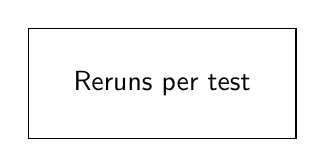
\begin{tikzpicture}
\draw (0,0) rectangle (3.4,1.4);
\node at (1.7,0.7) {\sffamily Reruns per test};
\end{tikzpicture}
\caption{The detector reruns each test in shuffled orders.}
\end{figure}
\lipsum[3-4]
\end{document}
